\documentclass[10pt,a4paper,sans]{moderncv} % Changed from 11pt to 10pt

\usepackage{amsfonts,amsthm,amsmath,amssymb,latexsym,xcolor,url}
\usepackage{graphicx,url,pifont,bbding,ifsym,textcomp}
\usepackage{multicol} % For two-column layout in research interests
\usepackage{fontawesome5} % For icons like location
\usepackage[scale=0.95, top=0.5cm, bottom=1.17cm]{geometry} % Adjust margins
\usepackage{fancyhdr} % For custom headers and footers
\usepackage{hyperref} % For clickable links


% Custom page number settings
\pagestyle{fancy}
\fancyhf{} % Clear header and footer
\renewcommand{\headrulewidth}{0pt} % Remove header rule
\renewcommand{\footrulewidth}{0.5pt} % Add footer rule
\fancyfoot[C]{\vspace{0.5cm}\textbf{\thepage}} % Center-align page numbers with spacing

% Disable default moderncv page numbers
\nopagenumbers

\moderncvstyle{classic}
\moderncvcolor{blue}

\renewcommand{\bfseries}{\fontseries{b}\selectfont}
\renewcommand{\itshape}{\fontshape{it}\selectfont}

% Adjust the font sizes of title and address
\renewcommand*{\titlefont}{\fontsize{12pt}{14pt}\selectfont} % Reduced from 14pt to 12pt
\renewcommand*{\addressfont}{\fontsize{8pt}{9pt}\selectfont} % Reduced from 9pt to 8pt

% Custom photo integration
\firstname{\textit{Bina}} % Your first name
\familyname{\textit{NiK}} % Your last name

\renewcommand*{\makecvtitle}{%
  \vspace*{-1.5cm} % Move the entire title block slightly up
  % Photo Section
  \begin{minipage}[t]{0.2\textwidth} % Adjust the width of the photo column
    \vspace*{0.5cm} % Add vertical space to move the photo down
    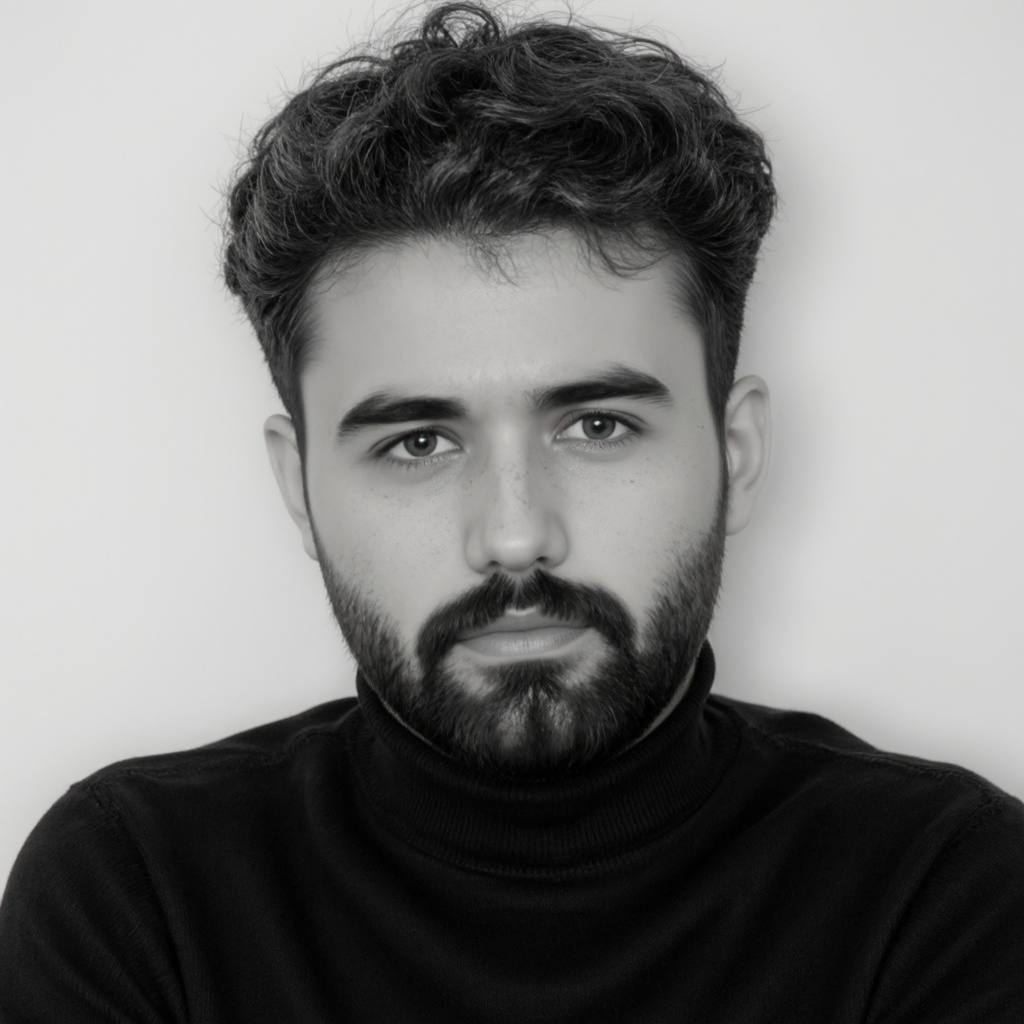
\includegraphics[width=2.9cm]{photo.jpg} % Explicitly set photo width
    \vspace*{-0.1cm}
  \end{minipage}
  \hfill
  % Text Section
  \begin{minipage}[t]{0.75\textwidth} % Adjust the width of the text column
    \vspace*{0.75cm} % Align the text to the top
    {\large\bfseries \firstname~\familyname}\\[-0.3ex] % Reduced from Large to large
    {\Large Ali NiK }\\[-3ex] % Reduced from Large to large
    \addressfont
    \begin{multicols}{2} % Start two-column layout
      \raggedright
      % Column 1
      
\includegraphics[height=1.8em]{house.png}\\ 
      \vspace{-0.43cm}\hspace{0.6cm}25C App.2.6.1,\\[0.5ex]
      \hspace{0.6cm}Vogeliusweg 25,\\[0.5ex]
      \hspace{0.6cm}33100 Paderborn, \\[0.5ex]
      \hspace{0.6cm}Nordrhein-Westfalen, \\[0.5ex]
      \hspace{0.6cm}Deutschland
      \\
      \columnbreak
      % Column 2
       
\includegraphics[height=1.4em]{iphone.png} {(+49) 0176 860 44654}\\[1ex]
       
\includegraphics[height=1.3em]{gmail.png} \href{mailto:ali.nazarikhah@iem.fraunhofer.de}{ali.nazarikhah@iem.fraunhofer.de}\\[1ex]
      
\includegraphics[height=1.3em]{linkedin.png} \href{https://linkedin.com/in/ali-nazarikhah}{https://linkedin.com/in/ali-nazarikhah}\\[1ex]
      
\includegraphics[height=1.3em]{github.png} \href{https://github.com/alinik24}{https://github.com/alinazarikhah}
    \end{multicols}
    \vspace*{-0.3cm}
  \end{minipage}
  % Add a horizontal line below the two sections
  \vspace*{-0.2cm}
  \line(1,0){557}

}

\begin{document}
\makecvtitle 




\section{\faGraduationCap{} AUSBILDUNG}

%Entry 1
\cvitem{
\raggedright
\makebox[5cm][l]{\footnotesize \faIcon{calendar-day} \colorbox{yellow!30}{2023/24 -- Heute}\hspace*{0.32cm}\textbf{MSc}} \\
\makebox[5cm][l]{\footnotesize\faMapMarker*{} 
\includegraphics[height=0.8em]{it.png} Italien / 
\includegraphics[height=0.8em]{de.png} Deutschland}
}{
$\bullet$ \textbf{Engineering in Computer Science [EiCS]} \newline 
{

\includegraphics[height=1.5em]{sap.png}\hspace{0.05em} 
\includegraphics[height=1.4em]{UPb.png} Fachbereich Informationsingenieurwesen, Informatik und Statistik, Sapienza Universität Rom / Universität Paderborn} \newline
{\scriptsize \faInfoCircle{}} \footnotesize Parallel zum MSc in Energy Engineering absolviert \newline% Changed small to footnotesize
{$\bullet$ \footnotesize Titel der Abschlussarbeit:} \footnotesize TBD
 \newline % Changed small to footnotesize
{$\bullet$ \footnotesize Betreuer:} \footnotesize TBD \newline % Changed small to footnotesize
{$\bullet$ \footnotesize GPA:} \footnotesize 90/110 [3.6/4.0 - alle Lehrveranstaltungen abgeschlossen; Abschlussarbeit ausstehend]
}
\vspace{0.25cm} 


% Entry 2
\cvitem{
\raggedright
\makebox[5cm][l]{\footnotesize\faIcon{calendar-day} 2022/23 -- 2025/26\hspace*{0.23cm}\textbf{MSc}} \\ % Changed small to footnotesize
\makebox[5cm][l]{\footnotesize\faMapMarker*{} 
\includegraphics[height=0.8em]{it.png} Italien}
}{
$\bullet$ \textbf{Energy Engineering [EE]} \newline
{
\includegraphics[height=1.5em]{sap.png} Fachbereich für Astronautik, Elektro- und Energietechnik, Sapienza Universität Rom} \newline
{$\bullet$ \footnotesize Titel der Abschlussarbeit:} \footnotesize Modellierung des Energiebedarfs industrieller Öfen zur Bewertung der Energieeffizienz;
Spezifikation und Validierung in einem Rollenherdofen
 \newline % Changed small to footnotesize
{$\bullet$ \footnotesize Betreuer:} \footnotesize Prof. Luigi Martirano \newline % Changed small to footnotesize
{$\bullet$ \footnotesize GPA:} \footnotesize 110/110 [4.0/4.0]
}
\vspace{0.25cm}

% Entry 3
\cvitem{
\raggedright
\makebox[5cm][l]{\footnotesize\faIcon{calendar-day} 2015/16 -- 2020/21\hspace*{0.23cm}\textbf{BSc}} \\ % Changed small to footnotesize
\makebox[5cm][l]{\footnotesize\faMapMarker*{} 
\includegraphics[height=0.8em]{ir.png} Iran}
}{
$\bullet$ \textbf{Chemical Engineering [CE]} \newline 
{

\includegraphics[height=1.5em]{Sahand University of Technology.png} Fachbereich Chemieingenieurwesen, Sahand University of Technology (SUT)} \newline
{$\bullet$ \footnotesize Titel der Abschlussarbeit:} \footnotesize Untersuchung der Auswirkungen elektrochemischer Prozesse und synthetisierter Zeolith-Nanoadsorbentien auf Membranverschmutzung in einem Membranbioreaktor \newline % Changed small to footnotesize
{$\bullet$ \footnotesize Betreuer:} \footnotesize Prof. Hossein Hazrati \newline % Changed small to footnotesize
{$\bullet$ \footnotesize GPA:} \footnotesize 18.06/20 [3.85/4.0] [4.0/4.0]
}

\section{\faGlobe{} FORSCHUNGSINTERESSEN}

\begin{multicols}{2}
\cvitem{}{\faBolt{} Energieumwandlung und Systemoptimierung}
\cvitem{}{\faSolarPanel{} Erneuerbare Energiesysteme und Nachhaltigkeit}
\cvitem{}{\faBuilding{} Intelligente Stromnetze und Energiesysteme in Smart Buildings}
\cvitem{}{\faCode{} Softwareentwicklung für Energieüberwachung, \newline Optimierung und vorausschauende Wartung}
\columnbreak
\cvitem{}{\faBrain{} KI- und ML-Anwendungen}
\cvitem{}{\faDatabase{} Datengetriebene Entscheidungsfindung}
\cvitem{}{\faMicrochip{} Internet der Dinge (IoT)}
\cvitem{}{\faCubes{} Blockchain-Anwendungen}
\cvitem{}{\faEdit{} UI/UX und Produktdesign}
\end{multicols}

\section{\faCogs{} BERUFSERFAHRUNG}

% GenAI Incubator entry
\cvitem{
\raggedright
\makebox[5cm][l]{\footnotesize \faIcon{calendar-day} \colorbox{yellow!30}{Mär 2025 -- Heute}} \\ % Changed small to footnotesize
\makebox[5cm][l]{\faMapMarker*{} \footnotesize Paderborn, Deutschland} % Changed small to footnotesize
}{$\bullet$ \textbf{Wissenschaftlicher Mitarbeiter} 
\newline{

\includegraphics[height=1.5em]{fraunhofer.png}\ GenAI Incubator, Fraunhofer IEM} \newline \footnotesize Durchführung von Forschung zu Generativer KI und ML-getriebenen Lösungen für industrielle Herausforderungen unter Nutzung datengetriebener Ansätze und Entscheidungsfindung zur Verbesserung von Automatisierung und operativer Effizienz.
} % Changed small to footnotesize

% Research Intern entry
\cvitem{
\raggedright
\makebox[5cm][l]{\footnotesize \faIcon{calendar-day} Feb 2024 -- Jun 2024} \\ % Changed small to footnotesize
\makebox[5cm][l]{\faMapMarker*{} \footnotesize Rom, Italien} % Changed small to footnotesize
}{$\bullet$ \textbf{Wissenschaftlicher Mitarbeiter}
\newline{

\includegraphics[height=0.9em]{enea.png}\ Energie- und Umwelttechnologie, Italienische Nationale Agentur für Neue Technologien (ENEA)} \newline \footnotesize Durchführung von Energieeffizienzbewertungen, Analyse der Integration erneuerbarer Energien, Entwicklung nachhaltiger Energielösungen und Mitwirkung an Forschung zu Emissionsminderungstechnologien im Einklang mit den Umweltzielen der EU.} % Changed small to footnotesize

% Energy Efficiency Consultant entry
\cvitem{
\raggedright
\makebox[5cm][l]{\footnotesize \faIcon{calendar-day} Jul 2021 -- Okt 2021} \\ % Changed small to footnotesize
\makebox[5cm][l]{\faMapMarker*{} \footnotesize Tabriz, Iran} % Changed small to footnotesize
}{$\bullet$ \textbf{Energieeffizienzberater} 
\newline{\scalebox{1.6}{\faIndustry}\ Talaaye Daaraane Moderne Shomal Gharb} \newline \footnotesize Durchführung industrieller Energieaudits, Analyse von Energieverbrauchsmustern, Vorschlag von Effizienzstrategien sowie Erstellung umsetzbarer Pläne zur Unterstützung nachhaltiger Entwicklung.} % Changed small to footnotesize

% Project Manager entry
\cvitem{
\raggedright
\makebox[5cm][l]{\footnotesize \faIcon{calendar-day} Mai 2021 -- Jun 2021} \\ % Changed small to footnotesize
\makebox[5cm][l]{\faMapMarker*{} \footnotesize Kharg Island, Iran} % Changed small to footnotesize
}{$\bullet$ \textbf{Projektsteuerungsingenieur} 
\newline{

\includegraphics[height=1.5em]{kharg.png}\ Kharg Petrochemical Company Limited} \newline \footnotesize Unterstützung des Projektmanagements während umfangreicher Revisionsarbeiten durch Terminverfolgung, Unterstützung der Ressourcenplanung, Sicherstellung der Einhaltung von HSE- und regulatorischen Vorgaben sowie Koordination multidisziplinärer Teams zur Erreichung der Projektmeilensteine.} % Changed small to footnotesize

% Process Engineering Technician entry
\cvitem{
\raggedright
\makebox[5cm][l]{\footnotesize \faIcon{calendar-day} Jan 2021 -- Apr 2021} \\ % Changed small to footnotesize
\makebox[5cm][l]{\faMapMarker*{} \footnotesize Mahshahr Port, Iran} % Changed small to footnotesize
}{$\bullet$ \textbf{Verfahrensingenieur} 
\newline{

\includegraphics[height=1.1em]{bandarimam.png}\ Bandar Imam Petrochemical Complex} \newline \footnotesize Verbesserung der Anlagenleistung durch Entwicklung präventiver Wartungsstrategien und Minimierung von Ausfallzeiten durch strukturierte Fehlerbehebung und Prozessanalyse.} % Changed small to footnotesize

\cvitem{
\raggedright
\makebox[5cm][l]{\footnotesize \faIcon{calendar-day} Jan 2017 -- Mär 2020} \\
\makebox[5cm][l]{\faMapMarker*{} \footnotesize Tabriz, Iran}
}{$\bullet$ \textbf{Wissenschaftlicher Mitarbeiter – Nachhaltige Verfahrenstechnik} 
\newline{

\includegraphics[height=1.5em]{Sahand University of Technology.png}\ Environmental Engineering Research Center (EERC), SUT} 
\newline \footnotesize Durchführung von Forschungsarbeiten im Bereich nachhaltiges industrielles Abfallmanagement sowie Entwicklung von Strategien zur Katalysatorregeneration und -synthese zur Nachbildung der Leistungsfähigkeit importierter Raffineriekatalysatoren unter Lieferengpässen.}

% Process Engineering Intern entry
\cvitem{
\raggedright
\makebox[5cm][l]{\footnotesize \faIcon{calendar-day} Jun 2017 -- Aug 2017} \\ % Changed small to footnotesize
\makebox[5cm][l]{\faMapMarker*{} \footnotesize Mohr, Iran} % Changed small to footnotesize
}{$\bullet$ \textbf{Praktikant Verfahrenstechnik} 
\newline{

\includegraphics[height=1.7em]{National_Iranian.png}\ Parsian Gas Refinery Company} \newline \footnotesize Erwerb von Fachkenntnissen in PFDs und P\&IDs, Bewertung von Raffinerieprozessen und Vorschlag von Energieeffizienzverbesserungen, einschließlich Forschung zur Rückgewinnung von Fackelgas und Prozesssimulationen.} % Changed small to footnotesize

\section{\faProjectDiagram{} PROJEKTE}

\cvitem{\faLaptopCode{} EiCS}{%
    $\bullet$ \textbf\footnotesize{Digitale Transformation des Projektmanagements bei Benteler — Digitalisierung von Legacy-Excel-Dateien, strukturierte Datenmodellierung, Aufbau einer zentralisierten Projektwissensbasis und Entwurf eines RAG-basierten Systems zur Informationsgewinnung.}
}

\cvitem{}{%
    $\bullet$ \textbf\footnotesize{Prädiktive Qualitätsmodellierung für SMT-Produktionslinien (FORVIA HELLA) — Entwicklung einer Machine-Learning-Pipeline zur frühzeitigen Fehlererkennung in der Leiterplattenfertigung unter Einsatz überwachter Lernverfahren und Explainable AI zur Klassifikation der Produktqualität sowie zur Bereitstellung nachvollziehbarer, interpretierbarer Entscheidungsunterstützung.}
}

\cvitem{}{%
    $\bullet$ \textbf\footnotesize{Digitalisierung elektrischer Schaltpläne für die industrielle Automatisierung (HIK) — Umwandlung elektrischer Schaltpläne in strukturierte, maschinenlesbare Schemata für Automatisierung, Interoperabilität und nachgelagerte ingenieurtechnische Integration.}
}

\cvitem{}{%
    $\bullet$ \textbf\footnotesize{Identifikation von Maschinenparametern und Datenmapping in der Batteriezellproduktion — Strukturierung, Optimierung und Konsistenzanalyse von Maschinenparametern zur Unterstützung skalierbarer digitaler Produktionsabläufe.}
}

\cvitem{}{%
    $\bullet$ \textbf\footnotesize{Entwicklung einer Legal-Tech-SaaS-Plattform (Konzept \& Prototyp) — Entwurf der Lösungsarchitektur, Definition von Service-Workflows und Skalierbarkeitsanalyse zur Automatisierung administrativer und juristischer Prozesse in Deutschland.}
}

\cvitem{}{%
    $\bullet$ \textbf\footnotesize{Anwendung zur physiognomiebasierten Persönlichkeitsanalyse — Entwicklung von Machine-Learning-Konzepten, UI/UX-Optimierung und interaktives Prototyping mit Figma.}
}

\cvitem{}{%
    $\bullet$ \textbf\footnotesize{Senior+ — KI-gesteuerte HR-Plattform — Entwurf adaptiver Onboarding- und Wissenssicherungs-Workflows unter Verwendung personalisierter, datengetriebener digitaler Prozesse.}
}

\cvitem{}{%
    $\bullet$ \textbf\footnotesize{Plattform zur Verwaltungsdigitalisierung für den öffentlichen Sektor — Entwurf eines digitalen Onboarding-Systems, Prozessautomatisierung, Usability-Optimierung und abteilungsübergreifende Workflow-Koordination.}
}

\cvitem{}{%
    $\bullet$ \textbf\footnotesize{Personalisierte Deep-Research-Plattform für Idea Scouting — Entwicklung eines datengetriebenen Forschungssystems für personalisierte Informationsgewinnung, strukturierte Marktanalyse und Evaluierung von Ideen in frühen Phasen.}
}


\vspace{0.25cm}

\cvitem{\faBolt{} EE}{%
    $\bullet$ \textbf\footnotesize{Techno-ökonomische Bewertung eines solarbetriebenen hybriden RO-MED-Entsalzungssystems in Bushehr, Iran.}
}

\cvitem{}{%
    $\bullet$ \textbf\footnotesize{Aerodynamische Optimierung von Windturbinenblättern mittels Computational Fluid Dynamics (Python/OpenFOAM).}
}

\cvitem{}{%
    $\bullet$ \textbf\footnotesize{Nachhaltige Energiewende durch Geothermie — Ressourcenbewertung, Anlagendesign und Machbarkeitsstudie für Lumut Balai, Indonesien (DoubleCalc 2D).}
}

\cvitem{}{%
    $\bullet$ \textbf\footnotesize{Entwurf eines Gezeitenenergie-Harvesters — Hydrodynamische Analyse und Leistungsprognose (OceanusLink).}
}

\cvitem{}{%
    $\bullet$ \textbf\footnotesize{Entwurf eines hybriden erneuerbaren Mikronetzes für ländliches Namibia — Resilienzanalyse unter extremen Wetterbedingungen (HOMER Pro/UQ).}
}

\cvitem{}{%
    $\bullet$ \textbf\footnotesize{Energieaudit und Optimierung am Campus X, Rom — Datengetriebene Echtzeit-Leistungsanalyse und mehrdimensionale Wirkungsbewertung.}
}

\cvitem{}{%
    $\bullet$ \textbf\footnotesize{DüsselPulse — KI-gesteuerte Smart-City-Lösungen in den Bereichen Energie, Wirtschaft, Mobilität, Umwelt und Gemeinschaft unter Nutzung datengetriebener Entscheidungsfindung und Unsicherheitsquantifizierung.}
}

\vspace{0.25cm}

\cvitem{\faIndustry{} CE}{%
    $\bullet$ \textbf\footnotesize{Techno-ökonomische Analyse und Optimierung der Wärmerückgewinnung von Festoxid-Elektrolyseuren für grünen Wasserstoff (PRO/II).}
}

\cvitem{}{%
    $\bullet$ \textbf\footnotesize{Optimierung von Fackelgasrückgewinnungssystemen in Raffinerien (Aspen HYSYS).}
}

\cvitem{}{%
    $\bullet$ \textbf\footnotesize{Businessplan für die katalytische Rückgewinnung auf Molekularsieb-Basis in der Adsorptionseinheit der Persian Gas Refinery — Anlagendesign und wirtschaftliche Bewertung.}
}

\cvitem{}{%
    $\bullet$ \textbf\footnotesize{Prozesssimulation und Optimierung der Reformer-Einheit im Kharg Petrochemical Complex (Aspen HYSYS).}
}

\cvitem{}{%
    $\bullet$ \textbf\footnotesize{CFD-Simulation von Rührbehältern — Vergleich von Turbulenzmodellen und Impeller-Designs mit COMSOL.}
}

\cvitem{}{%
    $\bullet$ \textbf\footnotesize{Simulation zweiphasiger Strömungen und Strategien zur verbesserten Förderung für das Arash-Gasfeld, Iran (ECLIPSE 300).}
}



\section{\faRocket{} KENNTNISSE}
\cvitem{\hspace*{-1cm}\textbf{\faBolt{} EE \& \faIndustry{} CE} \cvskill{4}}
{     
    \footnotesize Python (pvlib, Cantera, sympy), MATLAB, OpenFOAM, COMSOL Multiphysics, Aspen HYSYS, Pro/II , LabVIEW, PSS/E, HOMER Energy, Carrier HAP, Revit (BIM),    
    %EnergyPlus,    
    RETScreen Expert, PVsyst, KI-gesteuerte Industrieanalytik (Seeq), digitale Zwillinge (ANSYS Twin Builder), MS Project, %Jira,   
    Microsoft Office Suite %, Primavera P6
    }
    
\cvitem{\hspace*{0}\textbf{\faLaptopCode{} EiCS} \cvskill{2}}
{\footnotesize $\bullet$ \textbf{AI/ML Engineering} \hfill\cvskill{3} \newline 
LLMs, NLP, Generative KI (RAG, Diffusionsmodelle), %Multimodal AI,
PyTorch, TensorFlow, Hugging Face, LangChain, %Cloud AI Platforms (Vertex AI),
MLOps (MLflow, W\&B), Fine-Tuning \& Quantisierung, LM Studio, ComfyUI, n8n\newline
\footnotesize $\bullet$ \textbf{Data Science} \hfill\cvskill{2} \newline
Python (Polars, PySpark), R, SQL (inkl. BigQuery), %Snowflake, Apache Spark,
AutoML-Frameworks, DBT, Bildverarbeitung und Datenannotierungs-Workflows (Label Studio)
Jupyter \newline
\footnotesize $\bullet$ \textbf{Cloud \& Entwicklung} \hfill\cvskill{3} \newline
AWS, Azure, Docker/K8s, %React/Next.js,
FastAPI, KI-gestützte DevOps, Devin AI, Vercel, Expo, Figma, HTML5, CSS3}

\section{}
\vspace{-1cm}
\begin{center}
    \begin{minipage}[t]{0.5\textwidth} % Left Column (Workshops)
        \subsection{\faChalkboardTeacher{} WORKSHOPS \& ZERTIFIKATE} 
        \vspace{-0.1cm}
        \cvitem{
        \raggedright
        \makebox[5cm][l]{
\includegraphics[height=1em]{udd.png}Udemy}}{\footnotesize $\bullet$ KI-Agenten und fortgeschrittene Workflow-Automatisierung}
        \cvitem{}{\footnotesize $\bullet$ GenAI für Business Analysis: LLM Fine-Tuning und RAG-Architekturen}  
        \cvitem{
        \raggedright
        \makebox[5cm][l]{ 
\includegraphics[height=0.95em]{c.png} Coursera}}{\footnotesize $\bullet$ Deep Learning (Neuronale Netze, CNNs, Sequenzmodelle)} 
        \cvitem{}{\footnotesize $\bullet$ Verarbeitung natürlicher Sprache}
        \cvitem{}{\footnotesize $\bullet$ Sentimentanalyse mit Deep Learning} 
        \cvitem{}{\footnotesize $\bullet$ Game Design und Entwicklung}
        \cvitem{}{\footnotesize $\bullet$ Grundlagen des ethischen Hackings (EHE)} 
        \cvitem{}{\footnotesize $\bullet$ Web3 und Blockchain} 
        \cvitem{}{\footnotesize $\bullet$ Programmierung des Internets der Dinge (IoT)} 
        \cvitem{
        \raggedright
        \makebox[5cm][l]{ \faMapMarker*{} \footnotesize Kharg Island, Iran}}{\footnotesize $\bullet$ PFD- und P\&ID-Pläne in der Verfahrenstechnik, Kharg Petrochemical Complex} 
        \cvitem{}{\footnotesize $\bullet$ HSE-Grundsätze und -Praxis, Kharg Petrochemical Complex} 
    \end{minipage}%
    \hfill
    \begin{minipage}[t]{0.5\textwidth} % Right Column (Languages)
    \subsection{\faComments{} SPRACHEN} % No line under "Languages"

    \cvitem{}{\begin{tabular}{@{}p{2.8cm}@{\hskip 10pt}l}
        $\bullet$ Englisch   & \cvskill{5} \footnotesize C2 \\[0.5em]
        $\bullet$ Deutsch    & \cvskill{3} \footnotesize B1 \\[0.5em]
        $\bullet$ Italienisch& \cvskill{2} \footnotesize A2 \\[0.5em]
        $\bullet$ Arabisch   & \cvskill{2} \footnotesize A2 \\[0.5em]
        $\bullet$ Persisch   & \cvskill{5} \footnotesize C2 \\[0.5em]
        $\bullet$ Türkisch   & \cvskill{2} \footnotesize A2
    \end{tabular}}
\end{minipage}
\end{center}

\section{\faMedal{} AUSZEICHNUNGEN \& PREISE}

\cvitem{}{\footnotesize $\bullet$ Finalist, XChange4Industry Makeathon (Fraunhofer IEM) \newline
{\scriptsize (48-stündige Industrie-Challenge, die zu einem funktionsfähigen Prototypen für sicheren, souveränen und interoperablen Austausch von Fertigungsdaten führte, im Einklang mit den Prinzipien von Gaia-X und Factory-X.)}}

\cvitem{}{\footnotesize $\bullet$ Abschluss mit höchster Auszeichnung, MSc Energy Engineering, Sapienza Universität Rom \newline
{\scriptsize (Erster ausländischer Student, der parallel zwei ingenieurwissenschaftliche Masterstudiengänge absolvierte, dabei die volle Auszeichnung (110/110) innerhalb der Regelstudienzeit erreichte und im MSc-Programm Energy Engineering den ersten Platz im Jahrgang belegte.)}}



\cvitem{}{\footnotesize $\bullet$ Finalist beim Demo Day, DOCK3 Startup Incubator, Rom, Italien \newline
{\scriptsize (Eingebunden in ein dynamisches Startup-Ökosystem, wodurch praktische Erfahrungen in KI, ML, Edge Computing und aufkommenden digitalen Technologien gestärkt sowie Anpassungsfähigkeit und ein ausgeprägtes problemlösendes Denken gefördert wurden.)}}

\cvitem{}{\footnotesize $\bullet$ Platz 2 in meinem Jahrgang im BSc-Studiengang Chemical Engineering, Sahand University of Technology}

\cvitem{}{\footnotesize $\bullet$ Ausgezeichnet mit dem renommierten ``Financial Educational Award'' der National Elite Foundation des Iran}

\cvitem{}{\footnotesize $\bullet$ Unter den Top 1\% von 185.000 Teilnehmenden der iranischen nationalen Hochschulaufnahmeprüfung platziert und mit vollständigem Erlass der Studiengebühren für das Bachelorstudium ausgezeichnet}

\section{\faGamepad{} HOBBYS}

\begin{multicols}{3}
\cvitem{}{
\begin{tabular}{@{}l@{\hskip 10pt}l}
    \faYoutube{} \scriptsize Online-Lernen (YouTube, MOOCs) \\
    \faPodcast{} \scriptsize Technologische Innovationen \& Startup-Kultur \\ [-0.3em]
    \scriptsize newline (Nachrichten, Podcasts, Artikel)
    \end{tabular}}
\columnbreak
\cvitem{}{
\begin{tabular}{@{}l@{\hskip 10pt}l}
    \faBook{} \scriptsize Lesen \\
    \faChartLine{} \scriptsize Analyse der Finanzmärkte \\
\end{tabular}}
\columnbreak
\cvitem{}{
\begin{tabular}{@{}l@{\hskip 10pt}l}
     \faGuitar{} \scriptsize Klassische Gitarre \\
     \faDumbbell{} \scriptsize Fitness \& Sport
\end{tabular}}
\end{multicols}

\section{\faUser{} REFERENZEN 
\hfill {\normalsize \faFilePdf{}} \href{https://drive.google.com/file/d/1bWt9w5Vz_ohXiWX7r_eprzJ98oJn6Mc2/view?usp=drive_link}{\large{Empfehlungsschreiben}}
}


\vspace{0.65em}

% --- alignment control for email lines ---
\newcommand{\EmailAlign}{\hspace*{9 cm}}

\cvitem{Beruflich}{
\faBriefcase{} \textbf{Tommy Falkowski} \newline
Leiter des GenAI Incubator, Fraunhofer-Institut für Entwurfstechnik Mechatronik IEM, Paderborn, Deutschland \newline
\EmailAlign \faEnvelope{} \texttt{tommy.falkowski@iem.fraunhofer.de}
}
\vspace{0.25cm}

\cvitem{Akademisch--MSc}{
\faGraduationCap{} \textbf{Prof.\ Leonardo Micheli} \newline
Außerordentlicher Professor, Fachbereich für Astronautik, Elektro- und Energietechnik (DIAEE), Sapienza Universität Rom, Rom, Italien \newline
\EmailAlign \faEnvelope{} \texttt{leonardo.micheli@uniroma1.it}
}
\vspace{0.25cm}

\cvitem{Akademisch--BSc}{
\faGraduationCap{} \textbf{Prof.\ Mohammad Zabihi} \newline
Außerordentlicher Professor, Fachbereich Chemieingenieurwesen, Sahand University of Technology (SUT), Tabriz, Iran \newline
\EmailAlign \faEnvelope{} \texttt{zabihi@sut.ac.ir}
}
\vspace{0.25cm}

\cvitem{Beruflich}{
\faBriefcase{} \textbf{Eng.\ Mohammad Torabi} \newline
Direktor für Revisionsplanung und Projektsteuerung, Khark Petrochemical Complex, Khark Island, Iran \newline
\EmailAlign \faEnvelope{} \texttt{mohammad.torabi@khipc.com}
}

\end{document}